\documentclass[a4paper]{article}
\usepackage{latexsym}
\usepackage[a4paper]{geometry}
\usepackage{color}
\usepackage{listings}
\usepackage{subcaption}
\usepackage[pdftex]{graphicx}
\usepackage{subcaption}
\usepackage{hyperref}


\definecolor{Blue}{rgb}{0,0,0.5}
\definecolor{Green}{rgb}{0,0.75,0.0}
\definecolor{LightGray}{rgb}{0.6,0.6,0.6}
\definecolor{DarkGray}{rgb}{0.3,0.3,0.3}
\newcommand\matlabstyle{\lstset{language=Matlab,
   keywords={function,uint8,uint16,uint32,double,break,case,catch,continue,else,elseif,end,for,global,if,otherwise,persistent,return,switch,try,while},
   basicstyle=\ttfamily\footnotesize,
   breaklines=true,
   keywordstyle=\bfseries\color{Blue},
   commentstyle=\itshape\color{LightGray},
   stringstyle=\color{Green},
   numbers=left,
   numberstyle=\tiny\color{DarkGray},
   stepnumber=1,
   numbersep=10pt,
   backgroundcolor=\color{white},
   tabsize=2,
   showspaces=false,
   showstringspaces=false,
   captionpos=b}}

%Boldface text for type writer font
\usepackage{bold-extra} %\DeclareFontShape{OT1}{cmtt}{bx}{n}{<5><6><7><8><9><10><10.95><12><14.4><17.28><20.74><24.88>cmttb10}{}

%Break words properly at the end of a line (which isn't sloppy...)
\sloppy

% New definition of square root:
% it renames \sqrt as \oldsqrt
\let\oldsqrt\sqrt
% it defines the new \sqrt in terms of the old one
\def\sqrt{\mathpalette\DHLhksqrt}
\def\DHLhksqrt#1#2{%
\setbox0=\hbox{$#1\oldsqrt{#2\,}$}\dimen0=\ht0
\advance\dimen0-0.2\ht0
\setbox2=\hbox{\vrule height\ht0 depth -\dimen0}%
{\box0\lower0.4pt\box2}}

%Use command \exercise for each exercise
\newcounter{exerciseCount}
\setcounter{exerciseCount}{0}
\newcommand{\exercise}[1]{\addtocounter{exerciseCount}{1} \noindent \medskip {\large \textsf{\textbf{Exercise \arabic{exerciseCount} \--- #1}}} \par}
\renewcommand{\theenumi}{\textsf{\textbf{\alph{enumi}}}}

%Use command \code for code snippets
\newcommand{\code}[1]{\textnormal{\texttt{#1}}}

% Python environment
\lstnewenvironment{matlab}[1][]
{
\matlabstyle
\lstset{#1}
}
{}

% Python for external files
\newcommand\matlabexternal[2][]{{
\matlabstyle
\lstinputlisting[#1]{#2}}}

% Python for inline
\newcommand\matlabinline[1]{{\matlabstyle\lstinline!#1!}}
\usepackage{amsmath, amssymb, graphics, setspace}


\title{\textsf{Image Processing \\ Lab 2}}
\author{Han Kruiger(s1971190) \and Maarten Terpstra (s2028980)}
\date{\today}

\begin{document}
\maketitle
%!TEX root = report.tex
\exercise{Highboost filtering}
\setcounter{subsection}{0}

Sometimes it is desirable to highlight high-frequency components in an image without eliminating the low-frequency components.
One way to do this is by using a technique called highboost filtering.
This technique works by first blurring the image, then subtracting the blurred image from the original image - the result of this operation is called the mask - and then adding the mask to the original image.
Now edges are highlighted while retaining the same information about low-frequency components. 
\subsection{Implementation}
We have implemented the highboost filter in the function \texttt{IPhighboost}. We have set the blur mask to the same mask as in figure 3.32(a) as in the book, or as in table~\ref{tbl:mask}.
\begin{table}[!htb]
\begin{center}
$\frac{1}{9}$
\begin{tabular}{|c|c|c|}\hline
1 & 1 & 1 \\ \hline
1 & 1 & 1 \\ \hline
1 & 1 & 1 \\ \hline
\end{tabular}
\caption{The gaussian mask used for blurring}
\label{tbl:mask}
\end{center}
\end{table}
The following code implements the highboost filter operation (with \texttt{IPfilter} the same function as in the previous lab assignment):
\matlabexternal{IPhighboost.m}
When tested on the image \texttt{dipxetext.tif} the output for $k = 4.5$ gives the result of image~\ref{fig:dipxe}.
This is to our opinion the closest approximation of image 3.40(e) in the book.

\subsection{Negative values}
If an image \verb f  contains only positive values it is possible that the output image \verb g  contains negative values.
Consider the image described in table~\ref{tbl:inImage}. This image clearly contains only positive values. However, if is image is processed using \texttt{IPhighboost} with $k \geq 0.13$ the output image \verb g  will contain a negative value as table~\ref{tbl:outImage} illustrates.
We presume the minimal value of $k$ where negative values occur in the output image has a relation with the minimal value that occurs in the input image but we could not find strong evidence what this relation is. 

\begin{figure}[h]
 \centering
 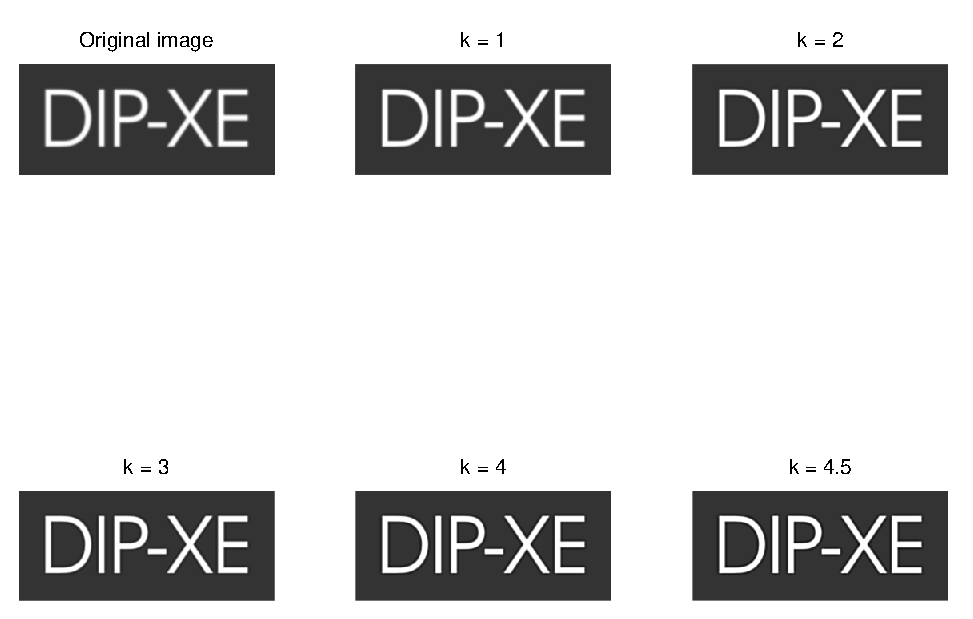
\includegraphics{dipxe.eps}
 \caption{Testing the highboost filter for several options of $k$. The image with $k = 4.5$, bottom-right, is the closest to image 3.40(e) in the book.}
 \label{fig:dipxe}
\end{figure}
\begin{table}[h]
  \begin{minipage}[b]{.5\linewidth}
    \centering
    \begin{tabular}{|c|c|c|}\hline
    1 & 1 & 1 \\ \hline
    1 & 0.1 & 1 \\ \hline
    1 & 1 & 1 \\ \hline
    \end{tabular}
    \subcaption{Input image}
    \label{tbl:inImage}
  \end{minipage}
  \hfill
  \begin{minipage}[b]{.5\linewidth}
    \centering
    \begin{tabular}{|c|c|c|}\hline
      1.3278 & 1.2167 & 1.3278 \\ \hline
      1.2167 & -0.3000 & 1.2167 \\ \hline
      1.3278 & 1.2167 & 1.3278 \\ \hline
    \end{tabular}
    \subcaption{Output image containing a negative value}
    \label{tbl:outImage}
  \end{minipage}
  \caption{The in- and output images for \texttt{IPhighboost}. It is clear that the output image contains negative values.}
  \hfill
\end{table}
\clearpage
%!TEX root = report.tex
\exercise{Texture}
\clearpage
%!TEX root = report.tex
\exercise{Wavelet denoising}
\subsection{Wavelet denoising implementation}
One of the interesting applications of the wavelet transform is performing noise reduction on images. Noise can be introduced in an image in a variety of ways and can be aesthetically pleasing or even necessary to remove it from an image to make it useful. Wavelet-based noise reduction algorithms may be more useful than other algorithms when noise must be reduces while features must be preserved. As noise is mostly present in the details of the wavelet transform, the wavelet transform is a good candidate to apply noise reduction when features must be preserved.

Noise is usually removed in the wavelet domain by applying thresholding to the details. However, this can be done in two ways: one can either \textit{hard} or \textit{soft} filtering. In the case of hard filtering, if the absolute value of a pixel is below a threshold value the pixel is set to zero. However, this can lead to discontinuity in an image. The alternative is applying so called soft thresholding which involves hard filtering and then scaling the non-zero components towards zero. 

We have implemented both ways of scaling in the function \texttt{IPwaveletdenoise} which allows an user to threshold the $J$-scale wavelet domain of an image with either hard or soft filtering. The function is implemented as following:
\matlabexternal{../IPwaveletdenoise.m}
The actual filtering is performed here:
\matlabexternal{../performFiltering.m}
The code performs exactly what it should do according to the description: it performs denoising by thresholding in the wavelet domain. 
\subsection{Denoising a noisy MRI image}
To ensure the code works we have executed the function on a noisy image in an attempt to denoise it. We have loaded \texttt{noisymri.tif}, which is a noisy MRI scan, in an attempt to denoise it. We have found out that a threshold value $t = 20$ is the best threshold value: it removes most of the noise while keeping most of the details. Figures~\ref{fig:noisyOrig} and~\ref{fig:noisyDenoise} illustrate the image before and after denoising with $t = 20$.
\begin{figure}[htb]
\centering
\begin{subfigure}{.5\textwidth}
  \centering
  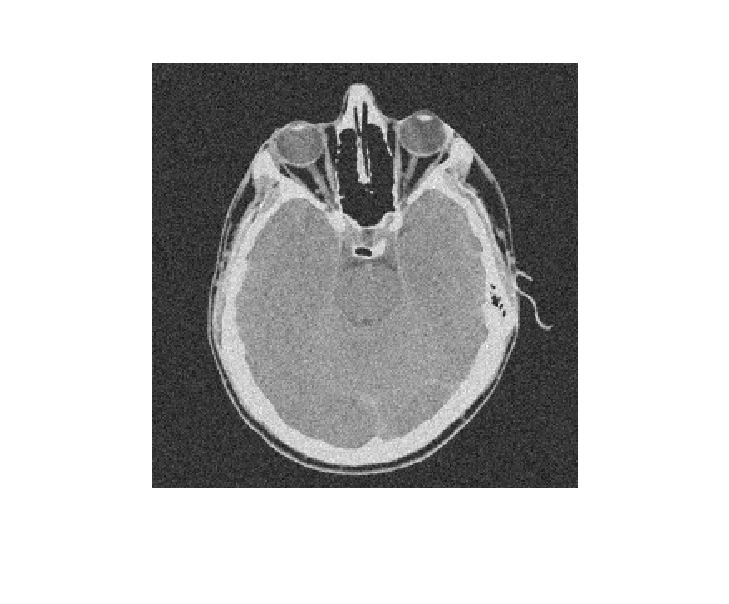
\includegraphics[scale=.7]{noisyMRI.eps}
  \caption{The original, noisy, MRI scan\newline}
  \label{fig:noisyOrig}
\end{subfigure}%
\centering
\begin{subfigure}{.5\textwidth}
  \centering
  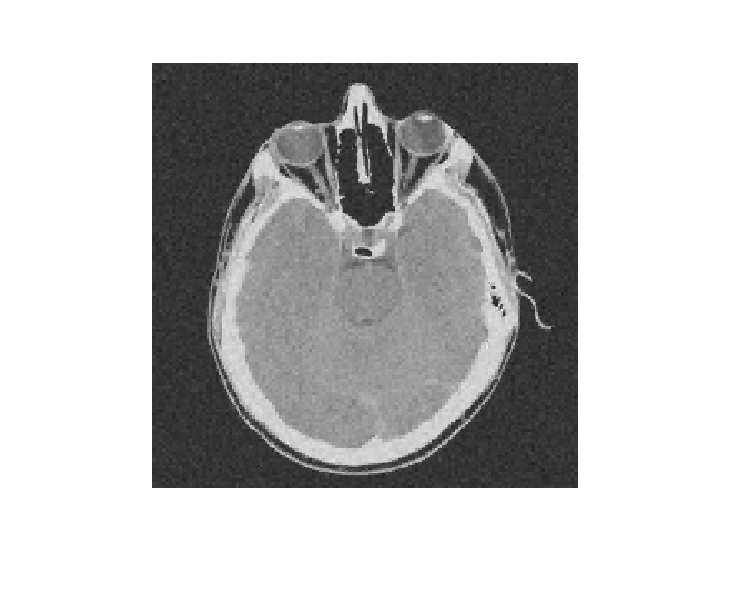
\includegraphics[scale=.7]{noisyMRI_Filtered.eps}
  \caption{The denoised image. Arguably, it is less noisy but the amount of detail is also lowered}
  \label{fig:noisyDenoise}
\end{subfigure}
\caption{An image of a MRI scan before and after denoising in the wavelet domain ($t = 2$, $j = 3$, $version = soft$)}
\label{fig:noiseReductionTest}
\end{figure}

Clearly, figure~\ref{fig:noisyDenoise} contains less noise than figure~\ref{fig:noisyOrig} while retaining most of its details. 
\clearpage
%!TEX root = report.tex
\addtocounter{exerciseCount}{1} \noindent \medskip {\large \textsf{\textbf{Workload distribution}}} \par
Here is table which describes our workload on this assignment per section. The overall percentage is how we feel we contributed individually to the entire assignment:

\begin{tabular}{ l | c | r }
    & Maarten & Han \\ \hline
  Programming & 50\% & 50\% \\
  \hline
  Exercise 1 report & 70\% & 30\% \\
  Exercise 2 report & 70\% & 30\% \\
  Exercise 3 report & 20\% & 80\% \\
  \hline
  Report overall & 50\% & 50\% \\ \hline \hline
  Overall & 50\% & 50\%
\end{tabular}
\bibliographystyle{unsrtnat}
\bibliography{references}
\end{document}
